\documentclass{article}

% if you need to pass options to natbib, use, e.g.:
% \PassOptionsToPackage{numbers, compress}{natbib}
% before loading nips_2017
%
% to avoid loading the natbib package, add option nonatbib:
% \usepackage[nonatbib]{nips_2017}

\usepackage[final]{nips_2017}

% to compile a camera-ready version, add the [final] option, e.g.:
% \usepackage[final]{nips_2017}

\usepackage[utf8]{inputenc} % allow utf-8 input
\usepackage[T1]{fontenc}    % use 8-bit T1 fonts
\usepackage{hyperref}       % hyperlinks
\usepackage{url}            % simple URL typesetting
\usepackage{booktabs}       % professional-quality tables
\usepackage{amsfonts}       % blackboard math symbols
\usepackage{nicefrac}       % compact symbols for 1/2, etc.
\usepackage{microtype}      % microtypography
\usepackage{graphicx}
\usepackage{amsmath}
\usepackage{float}
\usepackage{subfigure}

\title{Applying Compressive Sensing to the Cocktail Party Problem}

% The \author macro works with any number of authors. There are two
% commands used to separate the names and addresses of multiple
% authors: \And and \AND.
%
% Using \And between authors leaves it to LaTeX to determine where to
% break the lines. Using \AND forces a line break at that point. So,
% if LaTeX puts 3 of 4 authors names on the first line, and the last
% on the second line, try using \AND instead of \And before the third
% author name.

\author{
  Eli Saracino \\
  Department of Computer Science\\
  Boston University\\
  Boston, MA 02135 \\
  \texttt{esaracin@bu.edu} \\
  %% examples of more authors
  \And
  Andy Huynh \\
  Department of Computer Science \\
  Boston University \\
  Boston, MA 02135 \\
  \texttt{ndhuynh@bu.edu} \\
}



\begin{document}

\maketitle

\begin{abstract}
  A Compressed Sensing framework to approach blind source separation is investigated. We compare previous attempts, such as Nonnegative Matrix Factorization and Independent Component Analysis, and convey the potential advantages of Compressive Sensing: namely, it providing a more efficient reconstruction that relies far less on the necessity of learning.
\end{abstract}

\section{Introduction}
The applications of the Cocktail Party Problem are far-reaching: from surveying and separating radio signals, to imagining and examining neural signals in a medical setting, source separation plays an important role in an ever-expanding number of fields. An efficient approach to solving the Problem, then, has implications that extend far beyond the realm of Computer Science. 

Past techniques applied to solve this problem have, at a high level, relied largely on the learning of a specific dictionary, and the utilization of this dictionary to reconstruct distinct signals from potentially mixed sources. One such approach is Nonnegative Matrix Factorization, hereby NMF. As suggested, this method implies that prior information about speech sources is known in order to work properly, and, perhaps even more to its detriment, does not provide a well-defined solution in the case of over-complete dictionaries, which are so often utilized in the Compressive Sensing framework to minimize the number of measurements needed to reconstruct a given signal. \textbf{[1]} The NMF problem statement effectively tries to optimize the following cost function: 

\begin{figure}[H]
	\centering
	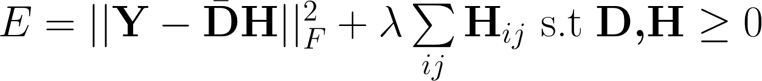
\includegraphics[width=250pt]{figs/NMF.png}
	\label{Nonnegative Matrix Factorization}
\end{figure}

where \textbf{$\bar{D}$} is a column-wise normalized dictionary matrix and \textbf{H} is the sparse solution upon which an $L_{1}$ norm penalty is induced. In keeping with the theme of NMF, both $\bar{D}$ and \textbf{H} must be nonnegative. In the above statement, $\lambda$ is a parameter that controls the degree of sparsity.

Notably, the problem statement is not totally dissimilar to that of the standard Compressive Sensing model, albeit with some minor differences. For example, the dictionary $\bar{D}$ must be learned, usually by training on a large dataset of a single speaker. This, of course, sacrifices efficiency and casts the framework of the reconstruction as a learning problem.  

With the advent of Compressive Sensing, however, we can model this problem in a new light. To do this, we first have make an assumption of sparsity; that is, in analyzing a mixed audio signal, at any given instant in time, we must assume that noise is coming from only a single source. In this way, the {\it frequency} domain of a mixed signal will be sparse, even if it should be the case that the the signal is quite robust in the time domain. With this assumption, we can frame the problem as a case of sparse signal recovery, defined as follows:

\begin{figure}[H]
	\centering
	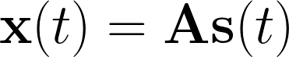
\includegraphics[width=94pt, height=15pt]{figs/compressive.png}
	\label{Compressive Sensing Problem Statement}
\end{figure}

where \textbf{S} is our set of source signals and \textbf{X} is a mixture of these signals as determined by our mixing matrix, \textbf{A}. As we will go on to show, determining \textbf{A} becomes a key step in the Compressive Sensing approach to solving the problem.

While solving this problem subject to the minimization the $L_{0}$ norm of \textbf{s} is notably NP-hard, we can obtain an approximate solution using any one of several greedy algorithms. Specifically, we apply Orthogonal Matching Pursuit to reconstruct the separate sparse signals, and transform them back into the time domain to complete the recovery.

In the coming sections, we will describe in more detail the compressive sensing approach used and it's computational benefits over such techniques as NMF, as well as some of its own shortcomings.


\section{Method}
The following is an overview of the algorithmic steps we take in applying Compressive Sensing to the Cocktail Party problem to reconstruct distinct signals from mixed input sources.

In the following steps, we'll assume we have a mixed signal of size \textit{T}. That is, there are \textit{T} discrete time instants over which our signal is heard.

In keeping with our assumption of a frequency-sparse input signal, the first step we take is to compute the Short-time Fourier transform of our source signal in order to cast it into its time-frequency domain. Shown below is a figure that demonstrates the utility of this transformation: an input signal that was originally robust becomes relatively sparse, with distinct structure forming along specific axes.

\begin{figure}[H]
	\centering
	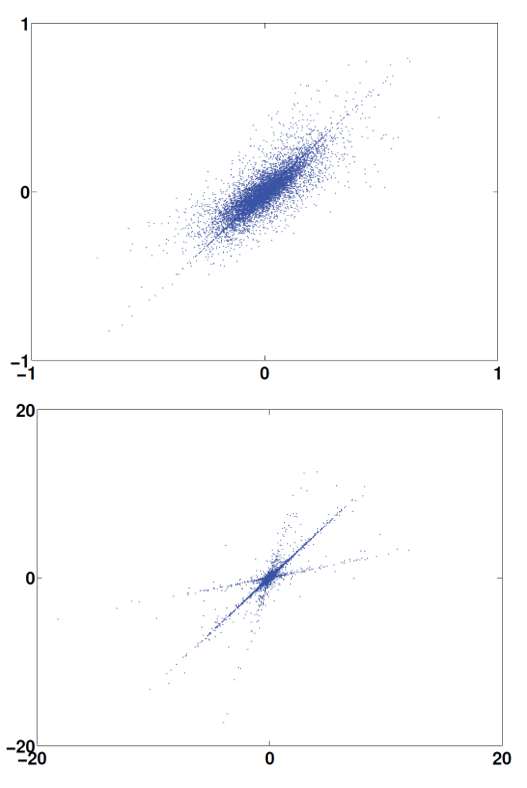
\includegraphics[width=180pt, height=220pt]{figs/transform_domain.png}
	\caption{Above, a mixed signal in the Time domain. Below, in the Transform domain \textbf{[1]}}
	\label{Signal in each Domain}
\end{figure}

It now becomes our job to generate a mixing matrix, defined as \textbf{A} in the Introduction's problem statement, in order to create a mixture of signals, \textbf{X}, that is able to be used in the reconstruction. The first step in this process it to apply k-means clustering to the normalized STFT computed in the previous step. By setting \textit{k} to the number of original sources we hope to separate, we are able to effectively partition the frequency domain of the transformed signal along the axes defined in the above figure.

Next, we use the one-dimensional cluster centers computed from the run of k-means to construct the mixing matrix. We'll define the following notation to express this process:

Let $C = \left( \begin{smallmatrix} c_{1}&c_{2}&...&c_{\textit{k}} \end{smallmatrix} \right)$ be the cluster centers previously computed. 

Let \textit{$L_{i}$} be a \textit{T} x \textit{T} diagonal matrix, of which there are \textit{k}, and whose diagonal entries are equivalent to the corresponding \textit{$i^{th}$} entry of \textit{C} as defined above.
 
We can finally define the mixing matrix \textit{M}, then, by concatenating these matrices horizontally, as follows: $M = \left( \begin{smallmatrix} L_{1}&L_{2}&...&L_{\textit{k}}  \end{smallmatrix} \right)$

As a final preparatory step, we multiply this matrix, \textit{M}, by a \textit{T} x \textit{T} DCT matrix to further sparsify the high-frequency components of human speech \textbf{[2]}. With this step, the preparation of our problem is complete, and the reconstruction of our separated signals can begin.

In practice, the reconstruction is often performed using a windowing method,as the dimensionality of the input signal, \textit{T}, can often be quite high, and the matrices described, then, can be quite large. Choosing some \textit{l} such that you compute the mixing matrix in \textit{l} x \textit{l} sections, and use it to reconstruct partial signals in a sectionalized way is a viable strategy, and it is what we employed in our reconstructions.

At each windowing phase, we perform Orthogonal Matching Pursuit to reconstruct the portion of the signal responsible for the window being processed. The concatenation of these windows together, then, yields the full, separated, original signal.


\section{Results}
In this section, we review the results of our reconstruction and compare it to other common methods of blind source separation. The main .wav file used for the tests was a mixture of Clint Eastwood and Graham speaking over each other. Other samples included data from the Interspeech 2006 source separation challenge, and are constructed of concise sentences following the same generally structure. The source .wav files were combined using the sox command line program. 

In practice, the results of using Compressive Sensing for blind source separation were underwhelming. The plots below depict the signal to noise ratio of our approach. In general, Independent Component Analysis, an industry standard of addressing the problem of blind source separation, is known to significantly outperform these results.


It's worth noting that

As can be seen, ICA provides a more accurate recovery than the Compressed Sensing approach, 

\begin{figure}[H]
  \centering
  \includegraphics[width=0.5\linewidth]{figs/Mixed" "Data.png}
  \caption{Sample figure caption.}
\end{figure}

\begin{figure}[H]
  \centering
  \subfigure[]{\includegraphics[width=0.49\linewidth]{figs/Recovered" "Source" "1.png}}
  \subfigure[]{\includegraphics[width=0.49\linewidth]{figs/Recovered" "Source" "2.png}}
  \caption{Sample figure caption.}
\end{figure}

\section*{References}

% References follow the acknowledgments. Use unnumbered first-level
% heading for the references. Any choice of citation style is acceptable
% as long as you are consistent. It is permissible to reduce the font
% size to \verb+small+ (9 point) when listing the references. {\bf
%   Remember that you can go over 8 pages as long as the subsequent ones contain
%   \emph{only} cited references.}
\medskip

\small

[1] Schmidt, Mikkel N. and Rasmus Kongsgaard Olsson. “Single-channel speech separation using sparse non-negative matrix factorization.” {\it INTERSPEECH} (2006).

[2] BAO, G., YE, Z., XU, X. AND ZHOU, Y.
{\it A Compressed Sensing Approach to Blind Separation of Speech Mixture Based on a Two-Layer Sparsity Model} - IEEE Journals \& Magazine Bao, G., Ye, Z., Xu, X. and Zhou, Y. (2017). A Compressed Sensing Approach to Blind Separation of Speech Mixture Based on a Two-Layer Sparsity Model - IEEE Journals \& Magazine. [online] Ieeexplore.ieee.org. Available at: http://ieeexplore.ieee.org/document/6384713/
\end{document}
